\documentclass[a4paper,11pt,twoside]{article}
\usepackage{a4wide}
\usepackage{multirow}
\usepackage{footnote}
\usepackage{amsbsy}
\usepackage[dvips]{graphicx}
\usepackage{fancyheadings}
%\setlength{\parindent}{0in}
%\setlength{\parskip}{0.05in}
\setlength{\parskip}{0.1in}


% set fancy headings

\pagestyle{fancy}
\lhead[{\it \thepage}]{{\bf\it {\tt wannier90}: Tutorial}}
\chead{}
\rhead[{\bf\it {\tt wannier90}: Tutorial}]{{\it \thepage}}
\setlength{\headrulewidth}{0.2pt}
\lfoot{}
\cfoot{}
\rfoot{}
\setlength{\footrulewidth}{0pt}
\setlength{\footskip}{0.25in}
\setlength{\parindent}{0in}

\title{\wannier: Tutorial}

\author{Version 1.0.3}
\date{3rd December 2007}

\begin{document}
\newcommand{\wannier}{\texttt{wannier90}}
\newcommand{\pwscf}{\textsc{pwscf}}
\newcommand{\QE}{\textsc{quantum-espresso}}
\newcommand{\Mkb}{\mathbf{M}^{(\mathbf{k},\mathbf{b})}}
\newcommand{\Ak}{\mathbf{A}^{(\mathbf{k})}}
\newcommand{\Uk}{\mathbf{U}^{(\mathbf{k})}}

\maketitle

\section*{Preliminaries}

Welcome to \wannier! The examples contained in this tutorial are
designed to help you to become familiar with the procedure of
generating, analysing and using maximally-localised Wannier functions
(MLWF). As a first step, install \wannier\ following the
instructions in the {\tt README} file of the \wannier\ distribution.
For an introduction to the theory underlying MLWF, you are encouraged
to refer to the brief overview given in the \wannier\ User
Guide~\cite{UserGuide}, to the two seminal papers of
Refs.~\cite{MV,SMV}, and to a recent paper~\cite{W90} describing
\wannier.

The following additional programs should be installed in order to
visualise the output of \wannier\ 
\begin{itemize}
\item {\tt gnuplot} is used to plot bandstructures. It is 
available for many operating systems and is often installed by default on
 unix/Linux distributions\\
{\tt http://www.gnuplot.info}
\item {\tt xmgrace} may also be used to plot bandstructures.\\
{\tt http://plasma-gate.weizmann.ac.il/Grace}
\item {\tt XCrySDen} is used to visualise crystal structures, MLWF,
  and Fermi surfaces. It is available for unix/Linux, 
  Windows (using cygwin), and OSX. To correctly display 
files from \wannier, version 1.4 or later must be used.\\
{\tt http://www.xcrysden.org}
\item {\tt vmd} can also be used to visualise crystal structures and
  MLWF.\\
{\tt http://www.ks.uiuc.edu/Research/vmd}
\end{itemize}



\section*{About this tutorial}

The first part of this tutorial comprises four examples taken from
Refs.~\cite{MV,SMV}: gallium arsenide, lead, silicon and copper. All
of the \wannier\ input files have been provided.

The second part of the tutorial covers the generation of \wannier\
input files starting from a full electronic structure calculation. We
have provided input files for the \pwscf\ ({\tt
  www.quantum-espresso.org}) interface to \wannier. Therefore, you
will need to install and compile elements of the {\tt
  quantum-espresso} package, namely {\tt pw.x} and {\tt
  pw2wannier90.x}, in order to run these
examples. Please visit {\tt www.quantum-espresso.org} to download the
package, and for installation instructions. 

At the time of
writing, interfaces to a number of other electronic structure codes,
such as {\sc 
  castep} ({\tt www.castep.org}), {\sc abinit} ({\tt
  www.abinit.org}), and {\sc fleur} ({\tt
  www.flapw.de}), are in progress.

For images of MLWF, see our gallery at {\tt
  http://www.wannier.org/gallery.html}. If you have any images that
  you would like to submit to the gallery, please email us at\\ {\tt 
  developers@wannier.org}.

\section*{Contact us}

If you have any suggestions regarding ways in which this tutorial may
be improved, then send us an email at {\tt
developers@wannier.org}. 

For other questions, email the \wannier\ forum at {\tt
  wannier@quantum-espresso.org}.  Note that first you will need to
register in order to post emails. Emails from non-registered users are
deleted automatically. You can register by following the links at\\
{\tt http://www.wannier.org/forum.html}.



\cleardoublepage

\section*{1: Gallium Arsenide}

\begin{itemize}
\item{Outline: \it{Obtain and plot MLWF for the four valence
    bands of GaAs.}} 
\item{Generation details: \it{From \pwscf, using norm-conserving
    pseudopotentials and a 2$\times$2$\times$2 k-point grid. Starting
    guess: four bond-centred Gaussians.}}
\item{Directory: {\tt examples/example1/}}
\item{Input Files}
\begin{itemize}
\item{ {\tt gaas.win}  {\it The master input file}}
\item{ {\tt gaas.mmn}  {\it The overlap matrices $\Mkb$}}
\item{ {\tt gaas.amn}  {\it Projection $\Ak$ of the Bloch states onto a set
    of trial localised orbitals}} 
\item{ {\tt UNK00001.1}  {\it The Bloch states in the real space unit
    cell. For plotting only.}} 
\end{itemize}
\end{itemize}

\begin{enumerate}
\item Run \wannier\ to minimise the MLWF spread
{\tt
\begin{quote}
wannier90.x gaas
\end{quote} }
Inspect the output file {\tt gaas.wout}. The total spread converges to its
minimum value after just a few iterations. Note that the geometric centre of
each MLWF lies along a Ga-As bond, slightly closer to As
than Ga. Note also that the memory requirement for the minimisation of
the spread is very low as the MLWF are defined at each
k-point by just the 4$\times$4 unitary matrices $\Uk$. 
\item Plot the MLWF by adding the following keywords to
  the input file {\tt gaas.win} 
{\tt
\begin{quote}
wannier\_plot = true
\end{quote} }
and re-running \wannier. To visualise the MLWF we must
represent them explicitly on a real space grid (see
Ref.~\cite{UserGuide}). As a consequence, plotting the MLWF is slower
and uses more memory than the minimisation of the spread. The four
files that are created ({\tt gaas\_00001.xsf}, etc.) can be viewed
using XCrySDen,\footnote{Once XCrySDen starts, click on {\tt Tools}
  $\rightarrow$ {\tt Data Grid} in order to specify an isosurface
  value to plot.} e.g.,
{\tt
\begin{quote}
xcrysden --xsf gaas\_00001.xsf
\end{quote} }

For large systems, plotting the MLWF may be time consuming
and require a lot of memory. Use the keyword {\tt wannier\_plot\_list}
to plot a subset of the MLWF. E.g., to plot the
1st, 2nd and 7th MLWF use 
{\tt
\begin{quote}
wannier\_plot\_list = 1 2 7
\end{quote} }
The MLWF are plotted in a supercell of the unit cell. The
size of this supercell is set through the keyword {\tt
  wannier\_plot\_supercell}. The default value is 2 (corresponding to a
supercell with eight times the unit cell volume). We recommend not using
values great than 3 as the memory and computational cost scales
cubically with supercell size.  

Plot the 3rd MLWF in a supercell of size 3. Choose a low
value for the isosurface (say 0.5). Can you explain what you see? 

{\it Hint:} For a finite k-point mesh, the MLWF are in fact
periodic and the period is related to the spacing of the k-point mesh. For
mesh with $n$ divisions in the $i^{\mathrm{th}}$ direction in the
Brillouin zone, the MLWF ``live'' in a supercell $n$ times the
unit cell. 
\end{enumerate}


\cleardoublepage



\section*{2: Lead}

\begin{itemize}
\item{Outline: \it{Obtain MLWF for the four lowest states
    in lead. Use Wannier interpolation to plot the Fermi surface}}
\item{Generation Details: \it{From \pwscf, using norm-conserving
    pseudopotentials and a 4$\times$4$\times$4 k-point grid. Starting
    guess: atom-centred sp$^3$ hybrid orbitals}} 
\item{Directory: {\tt examples/example2/}}
\item{Input Files}
\begin{itemize}
\item{ {\tt lead.win}  {\it The master input file}}
\item{ {\tt lead.mmn}  {\it The overlap matrices $\Mkb$}}
\item{ {\tt lead.amn}  {\it Projection $\Ak$ of the Bloch states onto a set
    of trial localised orbitals}} 
\item{ {\tt lead.eig}  {\it The Bloch eigenvalues at each k-point. For
    interpolation only}} 
\end{itemize}

\end{itemize}
The four lowest valence bands in lead are separated in energy from the
higher conduction states (see Fig.~\ref{fig:pb-bnd}). The MLWF of
these states have partial occupancy. MLWF describing only the occupied
states would be poorly localised.

\begin{enumerate}
\item Run \wannier\ to minimise the MLWF spread
{\tt
\begin{quote}
wannier90.x lead
\end{quote} }
Inspect the output file {\tt lead.wout}.
\item Use Wannier interpolation to obtain the Fermi surface of
  lead. Rather than re-running the whole calculation we can use the
  unitary transformations obtained in the first calculation and restart
  from the plotting routine. Add the following keywords to the {\tt
    lead.win} file: 
{\tt
\begin{quote}
restart = plot

fermi\_energy = 5.2676

fermi\_surface\_plot = true
\end{quote} }
and re-run \wannier. The value of the Fermi energy (5.2676\,eV) was
obtained from the initial first principles calculation. \wannier\
calculates the band energies, through wannier interpolation, on a 
dense mesh of k-points in the Brillouin zone. The density of this grid is
controlled by the keyword {\tt fermi\_surface\_num\_points}. The default
value is 50 (i.e., 50$^3$ points). 
The Fermi surface file {\tt lead.bxsf} can be viewed using XCrySDen,
e.g.,
{\tt
\begin{quote}
xcrysden --bxsf lead.bxsf
\end{quote} }
\end{enumerate}

\begin{figure}[h]
\begin{center}
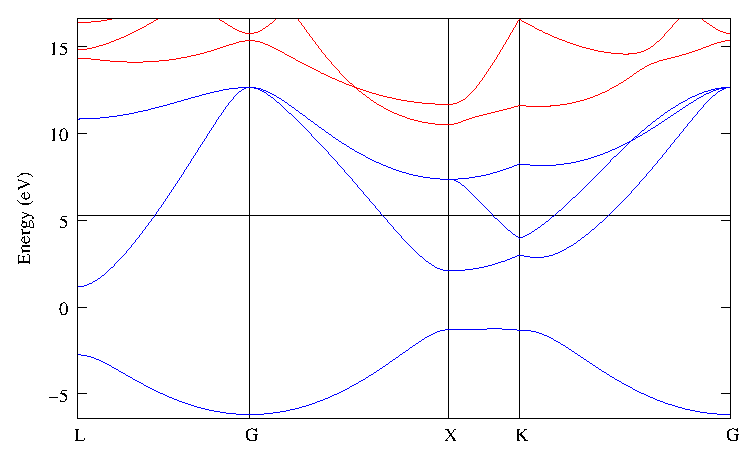
\includegraphics{lead.eps}
\caption{Bandstructure of lead showing the position of the Fermi
  level. Only the lowest four bands are included in the calculation.} 
\label{fig:pb-bnd}
\end{center}
\end{figure}

\cleardoublepage


\section*{3: Silicon}

\begin{itemize}
\item{Outline: \it{Obtain MLWF for the valence and low-lying
    conduction states of Si. Plot the interpolated bandstructure}} 
\item{Generation Details: \it{From \pwscf, using norm-conserving
    pseudopotentials and a 4$\times$4$\times$4 k-point grid. Starting
    guess: atom-centred sp$^3$ hybrid orbitals}} 
\item{Directory: {\tt examples/example3/}}
\item{Input Files}
\begin{itemize}
\item{ {\tt silicon.win}  {\it The master input file}}
\item{ {\tt silicon.mmn}  {\it The overlap matrices $\Mkb$}}
\item{ {\tt silicon.amn}  {\it Projection $\Ak$ of the Bloch states onto a
    set of trial localised orbitals}} 
\item{ {\tt silicon.eig}  {\it The Bloch eigenvalues at each k-point}}
\end{itemize}
\end{itemize}
The valence and lower conduction states can be represented by MLWF
with sp$^3$-like symmetry. The lower conduction states are not 
separated from the higher states by an energy gap. In order to form
localised WF, we use the disentanglement procedure
introduced in Ref.~\cite{SMV}. The position of the inner and outer
energy windows are shown in Fig.~\ref{fig:si.bnd}. 
\begin{enumerate}
\item Run \wannier.
{\tt
\begin{quote}
wannier90.x silicon
\end{quote} }
Inspect the output file {\tt silicon.wout}. The minimisation of the
spread occurs in a two-step procedure~\cite{SMV}. First, we minimise
$\Omega_{\rm I}$ -- this is the extraction of the optimal subspace in
the disentanglement procedure. Then, we minimise $\Omega_{\rm D} +
\Omega_{{\rm OD}}$.

\item Plot the MLWF by adding the following commands to
  the input file {\tt silicon.win} 
{\tt
\begin{quote}
restart = plot

bands\_plot = true
\end{quote} }
and re-running \wannier. The files {\tt silicon\_band.dat} and {\tt
  silicon\_band.gnu} are created. 
To plot the bandstructure using gnuplot
\smallskip
{\tt
\begin{quote}
myshell> gnuplot

gnuplot> load `silicon\_band.gnu'
\end{quote} }
The k-point path for the bandstructure interpolation is set in the {\tt
  kpoint\_path} block. Try plotting along different paths. 
\end{enumerate}

\begin{figure}[h]
\begin{center}
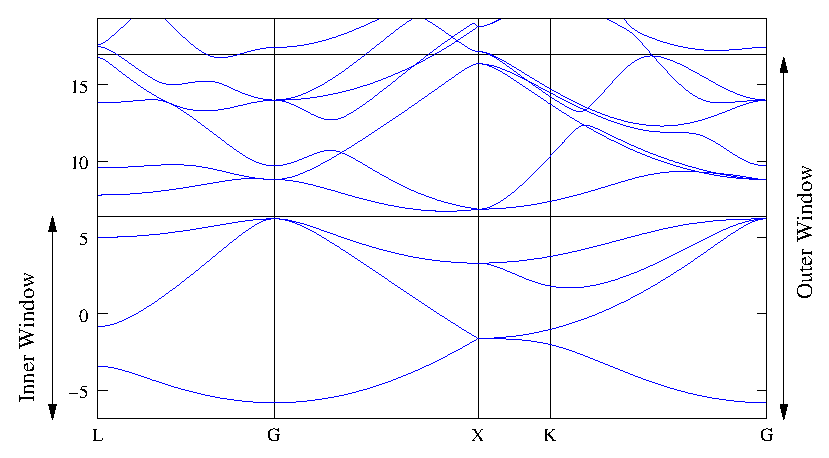
\includegraphics{si.eps}
\caption{Bandstructure of silicon showing the position of the outer
  and inner energy windows.} 
\label{fig:si.bnd}
\end{center}
\end{figure}

\cleardoublepage


\section*{4: Copper}

\begin{itemize}
\item{Outline: \it{Obtain MLWF to describe the states around the
    Fermi-level in copper}} 
\item{Generation Details: \it{From \pwscf, using ultrasoft
    pseudopotentials~\cite{USPP} and a
    4$\times$4$\times$4 k-point grid. Starting guess: five 
    atom-centred d orbitals, and two s orbitals centred on one of each
    of the two tetrahedral interstices.}}
\item{Directory: {\tt examples/example4/}}
\item{Input Files}
\begin{itemize}
\item{ {\tt copper.win}  {\it The master input file}}
\item{ {\tt copper.mmn}  {\it The overlap matrices $\Mkb$}}
\item{ {\tt copper.amn}  {\it Projection $\Ak$ of the Bloch states onto a
    set of trial localised orbitals}} 
\item{ {\tt copper.eig}  {\it The Bloch eigenvalues at each k-point}}
\end{itemize}

\end{itemize}

\begin{enumerate}
\item Run \wannier\ to minimise the MLWF spread
{\tt
\begin{quote}
wannier90.x copper
\end{quote} }
Inspect the output file {\tt copper.wout}. 

\item Plot the Fermi surface, it should look familiar! The Fermi
  energy is at 12.2103\,eV. 

\item Plot the interpolated bandstructure. A suitable path in k-space is
\smallskip
{\tt
\begin{quote}
begin kpoint\_path

G 0.00  0.00  0.00    X 0.50  0.50  0.00

X 0.50  0.50  0.00    W 0.50  0.75  0.25

W 0.50  0.75  0.25    L 0.00  0.50  0.00

L 0.00  0.50  0.00    G 0.00  0.00  0.00

G 0.00  0.00  0.00    K 0.00  0.50 -0.50
 
end kpoint\_path
\end{quote} }
\item Plot the contribution of the interstitial WF to the
  bandstructure. Add the following keyword to {\tt copper.win}
\smallskip
{\tt
\begin{quote}
bands\_plot\_project = 6,7
\end{quote} }
The resulting file {\tt copper\_band\_proj.gnu} can be opened with
gnuplot. Red lines correspond to a large contribution from the
interstitial WF (blue line are a small contribution; ie a large `d' contribution).


\end{enumerate}




Investigate the effect of the outer and inner energy window on the
interpolated bands. 



\begin{figure}[h]
\begin{center}
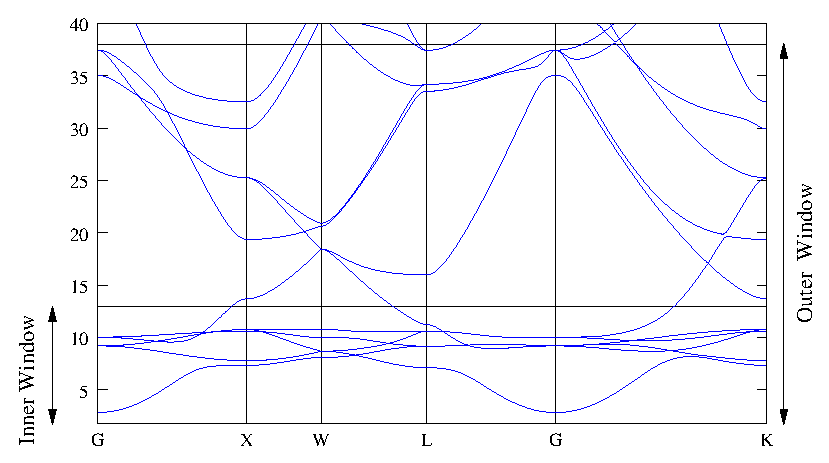
\includegraphics{cu.eps}
\caption{Bandstructure of copper showing the position of the outer
  and inner energy windows.} 
\label{fig:cu-bnd}
\end{center}
\end{figure}

\cleardoublepage

\begin{center}
\Large{\bf Examples Using the {\sc pwscf} Interface}
\end{center}

The \pwscf\ plane-wave, density-functional theory code, which is
available as part of the \QE\ distribution ({\tt
  www.quantum-espresso.org}), is fully interfaced to \wannier\ via the
{\tt pw2wannier90} post-processing code that is also available as part
of \QE. The latest version of {\tt pw2wannier90} is included as part of 
the \wannier\ distribution. Please see the {\tt pwscf} directory for 
instructions on how to incorporate it into \pwscf. 


\cleardoublepage

\section*{5: Diamond}
\begin{itemize}
\item{Outline: \it{Obtain MLWF for the valence bands of diamond}}
\item{Directory: {\tt examples/example5/}}
\item{Input Files}
\begin{itemize}
\item{ {\tt diamond.scf}  {\it The \pwscf\ input file for ground state
    calculation}} 
\item{ {\tt diamond.nscf}  {\it The \pwscf\ input file to obtain Bloch
    states on a uniform grid}} 
\item{ {\tt diamond.pw2wan}  {\it The input file for {\tt pw2wannier90}}}
\item{ {\tt diamond.win}  {\it The {\tt wannier90} input file}}
\end{itemize}
\end{itemize}

\begin{enumerate}
\item Run \pwscf\ to obtain the ground state of diamond\\
{\tt pw.x < diamond.scf > scf.out}

\item Run \pwscf\ to obtain the Bloch states on a uniform k-point grid\\
{\tt pw.x < diamond.nscf > nscf.out}

\item Run \wannier\ to generate a list of the required overlaps (written
  into the {\tt diamond.nnkp} file).\\ 
{\tt wannier90.x -pp diamond}

\item Run {\tt pw2wannier90} to compute the overlap between Bloch
  states and the projections for the starting guess (written in the
  {\tt diamond.mmn} and {\tt diamond.amn} files).\\  
{\tt pw2wannier90.x < diamond.pw2wan > pw2wan.out}

\item Run \wannier\ to compute the MLWF.\\
{\tt wannier90.x diamond}
\end{enumerate}

\cleardoublepage

\section*{6: Copper}

\begin{itemize}
\item{Outline: \it{Obtain MLWF to describe the states around the
    Fermi-level in copper}}
\item{Directory: {\tt examples/example6/}}
\item{Input Files}
\begin{itemize}
\item{ {\tt copper.scf}  {\it The \pwscf\ input file for ground state
    calculation}} 
\item{ {\tt copper.nscf}  {\it The \pwscf\ input file to obtain Bloch states
    on a uniform grid}} 
\item{ {\tt copper.pw2wan}  {\it Input file for {\tt pw2wannier90}}}
\item{ {\tt copper.win}  {\it The {\tt wannier90} input file}}
\end{itemize}

\end{itemize}

\begin{enumerate}
\item Run \pwscf\ to obtain the ground state of copper\\
{\tt pw.x < copper.scf > scf.out}

\item Run \pwscf\ to obtain the Bloch states on a uniform k-point grid\\
{\tt pw.x < copper.nscf > nscf.out}

\item Run \wannier\ to generate a list of the required overlaps (written
  into the {\tt copper.nnkp} file).\\ 
{\tt wannier90.x -pp copper}

\item Run {\tt pw2wannier90} to compute the overlap between Bloch
  states and the projections for the starting guess (written in the
  {\tt copper.mmn} and {\tt copper.amn} files).\\  
{\tt pw2wannier90.x < copper.pw2wan > pw2wan.out}

\item Run \wannier\ to compute the MLWF.\\
{\tt wannier90.x copper}
\end{enumerate}

Inspect the output file {\tt copper.wout}. 

\begin{enumerate}
\item Use Wannier interpolation to obtain the Fermi surface of
  copper. Rather than re-running the whole calculation we can use the
  unitary transformations obtained in the first calculation and restart
  from the plotting routine. Add the following keywords to the {\tt
    copper.win} file:
{\tt
\begin{quote}
restart = plot

fermi\_energy = [insert your value here] 

fermi\_surface\_plot = true
\end{quote} }
and re-run \wannier. The value of the Fermi energy can be  
obtained from the initial first principles calculation. \wannier\
calculates the band energies, through wannier interpolation, on a
dense mesh of k-points in the Brillouin zone. The density of this grid is
controlled by the keyword {\tt fermi\_surface\_num\_points}. The default
value is 50 (i.e., 50$^3$ points).
The Fermi surface file {\tt copper.bxsf} can be viewed using XCrySDen,
e.g., 
{\tt
\begin{quote}
xcrysden --bxsf copper.bxsf
\end{quote} }


\item Plot the interpolated bandstructure. A suitable path in k-space is
\smallskip
{\tt
\begin{quote}
begin kpoint\_path

G 0.00  0.00  0.00    X 0.50  0.50  0.00

X 0.50  0.50  0.00    W 0.50  0.75  0.25

W 0.50  0.75  0.25    L 0.00  0.50  0.00

L 0.00  0.50  0.00    G 0.00  0.00  0.00

G 0.00  0.00  0.00    K 0.00  0.50 -0.50
 
end kpoint\_path
\end{quote} }
\end{enumerate}

\subsection*{Further ideas}
\begin{itemize}
\item Compare the Wannier interpolated bandstructure with the full
  \pwscf\ bandstructure. Obtain MLWF using a more dense k-point grid.
\item Investigate the effect of the outer and inner energy window on
  the interpolated bands. 
\item Instead of extracting a subspace of seven states, we could extract a
  nine dimensional space (i.e., with s, p and d character). Examine this case
  and compare the projected bandstructures. 
\end{itemize}

%\begin{figure}[h]
%\begin{center}
%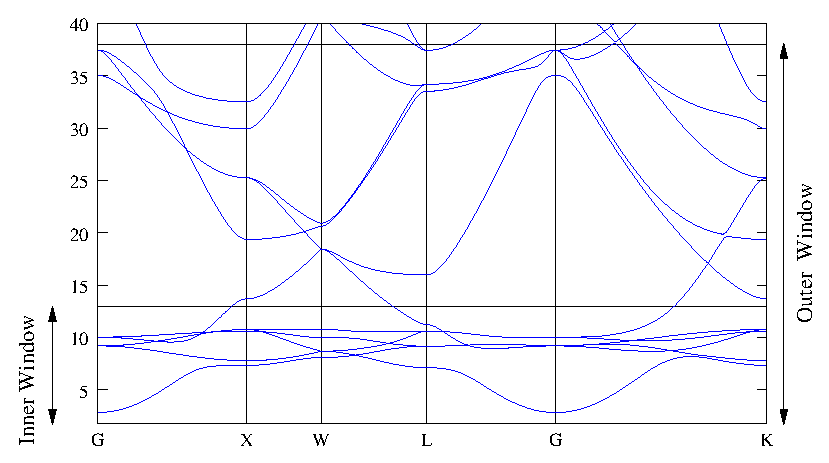
\includegraphics{cu.eps}
%\caption{Band Structure of Copper showing the position of the outer
%  and inner energy windows.}
%\label{fig:cu-bnd}
%\end{center}
%\end{figure}

\cleardoublepage

\section*{7: Silane - SiH$_4$}
\begin{itemize}
\item{Outline: \it{Obtain MLWF for the occupied states of molecular
    silane. $\Gamma$-point sampling}} 
\item{Directory: {\tt examples/example7/}}
\item{Input Files}
\begin{itemize}
\item{ {\tt silane.scf}  {\it The \pwscf\ input file for ground state
    calculation}} 
\item{ {\tt silane.nscf}  {\it The \pwscf\ input file to obtain Bloch states
    on a uniform grid}} 
\item{ {\tt silane.pw2wan}  {\it Input file for {\tt pw2wannier90}}}
\item{ {\tt silane.win}  {\it The {\tt wannier90} input file}}
\end{itemize}
\end{itemize}

\begin{enumerate}
\item Run \pwscf\ to obtain the ground state of silane\\
{\tt pw.x < silane.scf > scf.out}

\item Run \pwscf\ to obtain the Bloch states on a uniform k-point grid\\
{\tt pw.x < silane.nscf > nscf.out}

\item Run \wannier\ to generate a list of the required overlaps (written
  into the {\tt silane.nnkp} file).\\ 
{\tt wannier90.x -pp silane}

\item Run {\tt pw2wannier90} to compute the overlap between Bloch
  states and the projections for the starting guess (written in the
  {\tt silane.mmn} and {\tt silane.amn} files).\\  
{\tt pw2wannier90.x < silane.pw2wan > pw2wan.out}

\item Run \wannier\ to compute the MLWF.\\
{\tt wannier90.x silane}
\end{enumerate}

\cleardoublepage

\section*{8: Iron}
\begin{itemize}
\item{Outline: \it{Obtain MLWF to describe the states around the
    Fermi-level in iron.}} 
\item{Directory: {\tt examples/example8/}}
\item{Input Files}
\begin{itemize}
\item{ {\tt iron.scf}  {\it The \pwscf\ input file for ground state
    calculation}} 
\item{ {\tt iron.nscf}  {\it The \pwscf\ input file to obtain Bloch states
    on a uniform grid}} 
\item{ {\tt iron\_up.pw2wan}  {\it Input file for {\tt pw2wannier90} -
    spin up}} 
\item{ {\tt iron\_up.win}  {\it The {\tt wannier90} input file - spin up}}
\item{ {\tt iron\_dn.pw2wan}  {\it Input file for {\tt pw2wannier90} -
    spin down}} 
\item{ {\tt iron\_dn.win}  {\it The {\tt wannier90} input file - spin down}}
\end{itemize}
\item{Note that we obtain the MLWF for spin up and spin down in
  separate calculations.} 
\end{itemize}

\begin{enumerate}
\item Run \pwscf\ to obtain the ground state of iron\\
{\tt pw.x < iron.scf > scf.out}

\item Run \pwscf\ to obtain the Bloch states on a uniform k-point grid\\
{\tt pw.x < iron.nscf > nscf.out}

\item Run \wannier\ to generate a list of the required overlaps (written
  into the {\tt iron\_up.nnkp} and {\tt iron\_dn.nnkp} files).\\
{\tt wannier90.x -pp iron\_up}\\
{\tt wannier90.x -pp iron\_dn}

\item Run {\tt pw2wannier90} to compute the overlap between Bloch
  states and the projections for the starting guess (written in the
  {\tt iron\_up.mmn}, {\tt iron\_dn.mmn}, {\tt iron\_up.amn} and {\tt
  iron\_dn.amn} files).\\ 
{\tt pw2wannier90.x < iron\_up.pw2wan > pw2wan.out}\\
{\tt pw2wannier90.x < iron\_dn.pw2wan > pw2wan.out}

\item Run \wannier\ to compute the MLWF.\\
{\tt wannier90.x iron\_up}\\
{\tt wannier90.x iron\_dn}
\end{enumerate}


\cleardoublepage


\section*{9: Cubic BaTiO$_3$}
\begin{itemize}
\item{Outline: \it{Obtain MLWF for a perovskite}}
\item{Directory: {\tt examples/example9/}}
\item{Input Files}
\begin{itemize}
\item{ {\tt batio3.scf}  {\it The \pwscf\ input file for ground state
    calculation}} 
\item{ {\tt batio3.nscf}  {\it The \pwscf\ input file to obtain Bloch states
    on a uniform grid}} 
\item{ {\tt batio3.pw2wan}  {\it Input file for {\tt pw2wannier90}}}
\item{ {\tt  batio3.win}  {\it The {\tt wannier90} input file}}
\end{itemize}
\end{itemize}

 To start with, we are going to obtain MLWF for the oxygen 2p
  states. From the bandstructure~\cite{BaTiO3}, these form an isolated
  group of bands. We use the \wannier\ keyword {\tt exclude\_bands} to
  remove all but the 2p bands from the calculation of the overlap
  and projection matrices (we don't have to do this, but it saves time).

\begin{enumerate}
\item Run \pwscf\ to obtain the ground state of BaTiO$_3$\\
{\tt pw.x < BaTiO3.scf > scf.out}

\item Run \pwscf\ to obtain the Bloch states on a uniform k-point grid\\
{\tt pw.x < BaTiO3.nscf > nscf.out}

\item Run \wannier\ to generate a list of the required overlaps (written
  into the {\tt BaTiO3.nnkp} file).\\ 
{\tt wannier90.x -pp BaTiO3}

\item Run {\tt pw2wannier90} to compute the overlap between Bloch
  states and the projections for the starting guess (written in the
  {\tt BaTiO3.mmn} and {\tt BaTiO3.amn} files).\\  
{\tt pw2wannier90.x < BaTiO3.pw2wan > pw2wan.out}

\item Run \wannier\ to compute the MLWF.\\
{\tt wannier90.x BaTiO3}
\end{enumerate}

Inspect the output file {\tt BaTiO3.wout}. 

Plot the second MLWF, as described in Section~1, by adding the
following keywords to the input file {\tt BaTiO3.win}
{\tt
\begin{quote}
wannier\_plot = true\\
restart = plot\\
wannier\_plot\_list = 2\\
wannier\_plot\_supercell = 3
\end{quote} }
and re-running \wannier. Visualise it using XCrySDen,
{\tt
\begin{quote}
xcrysden --xsf BaTiO3\_00002.xsf
\end{quote} }

We can now simulate the ferroelectric phase by displacing the Ti
  atom. Change its position to 
{\tt
\begin{quote}
Ti 0.505 0.5 0.5
\end{quote}
}
and regenerate the MLWF (i.e., compute the ground-state charge
density and Bloch states using \pwscf, etc.) and look at the change in
the second MLWF.

\subsection*{Further ideas}
\begin{itemize}
\item Look at MLWF for other groups of bands. What happens if you form
  MLWF for the whole valence manifold?

\item Following Ref.~\cite{BaTiO3}, compute the Born effective charges from the
  change in Wannier centres under an atomic displacement. 
\end{itemize}

\cleardoublepage

\section*{10: Graphite}
\begin{itemize}
\item{Outline: \it{Obtain MLWF for graphite (AB, Bernal)}}
\item{Directory: {\tt examples/example10/}}
\item{Input Files}
\begin{itemize}
\item{ {\tt graphite.scf}  {\it The \pwscf\ input file for ground
    state calculation}} 
\item{ {\tt graphite.nscf}  {\it The \pwscf\ input file to obtain Bloch
    states on a uniform grid}} 
\item{ {\tt graphite.pw2wan}  {\it Input file for {\tt pw2wannier90}}}
\item{ {\tt graphite.win}  {\it The {\tt wannier90} input file}}
\end{itemize}
\end{itemize}

\begin{enumerate}
\item Run \pwscf\ to obtain the ground state of graphite\\
{\tt pw.x < graphite.scf > scf.out}

\item Run \pwscf\ to obtain the Bloch states on a uniform k-point grid\\
{\tt pw.x < graphite.nscf > nscf.out}

\item Run \wannier\ to generate a list of the required overlaps (written
  into the {\tt graphite.nnkp} file).\\ 
{\tt wannier90.x -pp graphite}

\item Run {\tt pw2wannier90} to compute the overlap between Bloch
  states and the projections for the starting guess (written in the
  {\tt graphite.mmn} and {\tt graphite.amn} files).\\  
{\tt pw2wannier90.x < graphite.pw2wan > pw2wan.out}

\item Run \wannier\ to compute the MLWF.\\
{\tt wannier90.x graphite}
\end{enumerate}


\cleardoublepage


\section*{11: Silicon}
\subsection*{Valence Bands}
\begin{itemize}
\item{Outline: \it{Obtain MLWF for the valence bands of silicon}}
\item{Directory: {\tt examples/example11/}}
\item{Input Files}
\begin{itemize}
\item{ {\tt silicon.scf}  {\it The \pwscf\ input file for ground state
    calculation}} 
\item{ {\tt silicon.nscf}  {\it The \pwscf\ input file to obtain Bloch
    states on a uniform grid}} 
\item{ {\tt silicon.pw2wan}  {\it Input file for {\tt pw2wannier90}}}
\item{ {\tt silicon.win}  {\it The {\tt wannier90} input file}}
\end{itemize}

\end{itemize}

\begin{enumerate}
\item Run \pwscf\ to obtain the ground state of silicon\\
{\tt pw.x < silicon.scf > scf.out}

\item Run \pwscf\ to obtain the Bloch states on a uniform k-point
  grid. Note that we request the lower 4 (valence) bands\\ 
{\tt pw.x < silicon.nscf > nscf.out}

\item Run \wannier\ to generate a list of the required overlaps (written
  into the {\tt silicon.nnkp} file).\\
{\tt wannier90.x -pp silicon}

\item Run {\tt pw2wannier90} to compute the overlap between Bloch
  states and the projections for the starting guess (written in the
  {\tt silicon.mmn} and {\tt  silicon.amn} files).\\
{\tt pw2wannier90.x < silicon.pw2wan > pw2wan.out}

\item Run \wannier\ to compute the MLWF.\\
{\tt wannier90.x silicon}

\end{enumerate}

Inspect the output file {\tt silicon.wout}. The total spread converges to its
minimum value after just a few iterations. Note that the geometric centre of
each MLWF lies at the centre of the Si-Si bond.
Note also that the memory requirement for the minimisation of
the spread is very low as the MLWF are defined 
by just the 4$\times$4 unitary matrices $\Uk$. 

Plot the MLWF by adding the following keywords to the input file {\tt
  silicon.win} 
{\tt
\begin{quote}
wannier\_plot = true
\end{quote} }
and re-running \wannier. Visualise them using XCrySDen, e.g.,
{\tt
\begin{quote}
xcrysden --xsf silicon\_00001.xsf
\end{quote} }

\subsection*{Valence + Conduction State}

\begin{itemize}
\item{Outline: \it{Obtain MLWF for the valence and low-lying
    conduction states of Si. Plot the interpolated bandstructure}} 
\item{Input Files}
\begin{itemize}
\item{ {\tt silicon.scf}  {\it The \pwscf\ input file for ground state
    calculation}} 
\item{ {\tt silicon.nscf}  {\it The \pwscf\ input file to obtain Bloch
    states on a uniform grid}} 
\item{ {\tt silicon.pw2wan}  {\it Input file for {\tt pw2wannier90}}}
\item{ {\tt silicon.win}  {\it The {\tt wannier90} input file}}
\end{itemize}
\end{itemize}
The valence and lower conduction states can be represented by MLWF
with sp$^3$-like symmetry. The lower conduction states are not 
separated by an energy gap from the higher states. In order to form
localised WF we use the disentanglement procedure
introduced in Ref.~\cite{SMV}. The position of the inner and outer
energy windows are shown in Fig.~\ref{fig:si.bnd}. 
\begin{enumerate}
\item Modify the input file and run \pwscf\ and \wannier.\\
Inspect the output file {\tt silicon.wout}. The minimisation of the
spread occurs in a two-step procedure. First, we minimise $\Omega_{\rm
  I}$ -- this is the extraction of the optimal subspace in the 
disentanglement procedure. Then, we minimise $\Omega_{\rm
  O}+\Omega_{{\rm OD}}$.

\item Plot the bandstructure by adding the following commands to the
 input file {\tt silicon.win}
{\tt
\begin{quote}
restart = plot

bands\_plot = true
\end{quote} }
and re-running \wannier. The files {\tt silicon\_band.dat} and {\tt
  silicon\_band.gnu} are created. To plot the bandstructure using
  gnuplot \smallskip
{\tt
\begin{quote}
myshell> gnuplot

gnuplot> load `silicon\_band.gnu'
\end{quote} }
The k-point path for the bandstructure interpolation is set in the {\tt
  kpoint\_path} block. Try plotting along different paths. 
\end{enumerate}

\subsection*{Further ideas}

\begin{itemize}
\item Compare the Wannier interpolated bandstructure with the full
  \pwscf\ bandstructure. Compute MLWF using a finer
  k-point grid (e.g., 6$\times$6$\times$6 or 8$\times$8$\times$8) and
  note how the accuracy of the interpolation increases~\cite{WanInt}.
\item Compute MLWF for four conduction states (see Ref.~\cite{SMV}).
\end{itemize}

%\begin{figure}[h]
%\begin{center}
%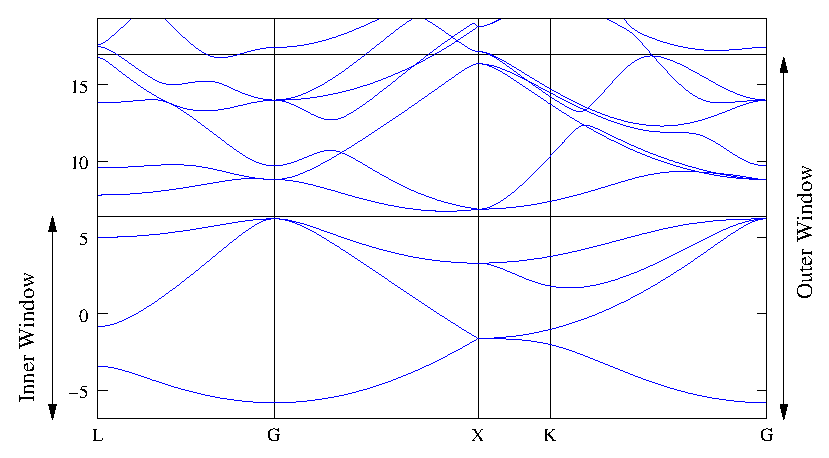
\includegraphics{si.eps}
%\caption{Band Structure of Silicon showing the position of the outer
%and inner energy windows.}
%\label{fig:si.bnd}
%\end{center}
%\end{figure}

\cleardoublepage


\section*{12: Benzene}
\subsection*{Valence States}
\begin{itemize}
\item{Outline: \it{Obtain MLWF for the valence states of benzene}}
\item{Directory: {\tt examples/example12/}}
\item{Input Files}
\begin{itemize}
\item{ {\tt benzene.scf}  {\it The \pwscf\ input file for ground state
    calculation}} 
\item{ {\tt benzene.pw2wan}  {\it Input file for {\tt pw2wannier90}}}
\item{ {\tt benzene.win}  {\it The {\tt wannier90} input file}}
\end{itemize}

\end{itemize}

\begin{enumerate}
\item Run \pwscf\ to obtain the ground state of benzene\\
{\tt pw.x < benzene.scf > scf.out}

\item Run \wannier\ to generate a list of the required overlaps (written
  into the {\tt benzene.nnkp} file).\\
{\tt wannier90.x -pp benzene}

\item Run {\tt pw2wannier90} to compute the overlap between Bloch
  states and the projections for the starting guess (written in the
  {\tt benzene.mmn} and {\tt  benzene.amn} files).\\
{\tt pw2wannier90.x < benzene.pw2wan > pw2wan.out}

\item Run \wannier\ to compute the MLWF.\\
{\tt wannier90.x benzene}

\end{enumerate}

Inspect the output file {\tt benzene.wout}. The total spread converges
to its minimum value after just a few iterations. 

Plot the MLWF by adding the following keywords to the input file {\tt
  benzene.win} 
{\tt
\begin{quote}
restart               = plot\\
wannier\_plot         = true\\
wannier\_plot\_format = cube\\
wannier\_plot\_list   = 2-4
\end{quote} }
and re-running \wannier. Visualise them using, e.g., XCrySDen. 

\subsection*{Valence + Conduction States}

\begin{itemize}
\item{Outline: \it{Obtain MLWF for the valence and low-lying
    conduction states of benzene.}} 
\item{Input Files}
\begin{itemize}
\item{ {\tt benzene.scf}  {\it The \pwscf\ input file for ground state
    calculation}} 
\item{ {\tt benzene.nscf}  {\it The \pwscf\ input file to obtain Bloch
    states for the conduction states}} 
\item{ {\tt benzene.pw2wan}  {\it Input file for {\tt pw2wannier90}}}
\item{ {\tt benzene.win}  {\it The {\tt wannier90} input file}}
\end{itemize}
\end{itemize}
In order to form localised WF we use the disentanglement
procedure. The position of the inner energy window is set to lie in
the energy gap; the outer energy window is set to 4.0\,eV. Modify the
input file appropriately. 
\begin{enumerate}
\item Run \pwscf\ and \wannier.\\
Inspect the output file {\tt benzene.wout}. The minimisation of the
spread occurs in a two-step procedure. First, we minimise $\Omega_{\rm
  I}$. Then, we minimise $\Omega_{\rm O}+\Omega_{{\rm OD}}$.

\item Plot the MLWF by adding the following commands to the
 input file {\tt benzene.win}
{\tt
\begin{quote}
restart               = plot\\
wannier\_plot         = true\\
wannier\_plot\_format = cube\\
wannier\_plot\_list   = 1,7,13
\end{quote} }
and re-running \wannier. Visualise them using, e.g., XCrySDen. 
\end{enumerate}

\cleardoublepage


\section*{13: (5,5) Carbon Nanotube}
\subsection*{Transport properties}

\begin{itemize}
  \item{Outline: \it{Obtain the bandstructure, quantum conductance and
  density of states of a metallic (5,5) carbon nanotube}}
  \item{Directory: {\tt examples/example13/}}
  \item{Input Files}
    \begin{itemize}
      \item{ {\tt cnt55.scf}  {\it The \pwscf\ input file for ground state
	  calculation}}
      \item{ {\tt cnt55.nscf}  {\it The \pwscf\ input file to obtain Bloch
	  states for the conduction states}} 
      \item{ {\tt cnt55.pw2wan}  {\it Input file for {\tt pw2wannier90}}}
      \item{ {\tt cnt55.win}  {\it The {\tt wannier90} input file}}
    \end{itemize}
\end{itemize}

In order to form localised WF that describe both the occupied and
unoccupied $\pi$ and $\pi^{\ast}$ manifolds, we use the
disentanglement procedure to extract a smooth manifold of states that
has dimension equal to 2.5 times the number of carbon atoms per unit
cell~\cite{WanTran}. The positions of the energy windows are shown in
Fig.~\ref{fig:cnt.win}.

The part of the \wannier\ input file that controls the transport part
of the calculation looks like:

{\tt
\begin{quote}
transport                 = true\\
transport\_mode           = bulk\\
one\_dim\_axis            = z\\
dist\_cutoff              =  5.5\\
fermi\_energy             = -1.06\\
tran\_win\_min            = -6.5\\
tran\_win\_max            = 6.5\\
tran\_energy\_step         = 0.01\\
dist\_cutoff\_mode        = one\_dim\\
translation\_centre\_frac = 0.0 0.0 0.0
\end{quote} }

Descriptions of these and other keywords related to the calculation of
transport properties can be found in the User Guide.

\begin{enumerate}
\item Run \pwscf\ and \wannier.\\
Inspect the output file {\tt cnt55.wout}. The minimisation of the
spread occurs in a two-step procedure. First, we minimise $\Omega_{\rm
  I}$. Then, we minimise $\Omega_{\rm O}+\Omega_{{\rm OD}}$.
\item Note that the initial $p_{z}$ projections on the carbon atoms
are oriented in the radial direction with respect to the nanotube
axis.
\item The interpolated bandstructure is written to {\tt
cnt55\_band.agr} (since {\tt bands\_plot\_format = xmgr} in the input
file).
\item The quantum conductance and density of states are written to the
files {\tt cnt55\_qc.dat} and {\tt cnt55\_dos.dat}, respectively. 
Note that this part of the calculation may take some time. You can 
follow its progress by monitoring the output to these files. 
Use a package such as {\tt gnuplot} or {\tt xmgrace} in order to visualise
the data. You should get something that looks like Fig.~\ref{fig:cnt.tran}.
\end{enumerate}

\begin{figure}[h]
\begin{center}
\scalebox{0.75}{\includegraphics{cnt.win.eps}}
\caption{Bandstructure of (5,5) carbon nanotube showing the position
  of the outer and inner energy windows.}
\label{fig:cnt.win}
\end{center}
\end{figure}

\begin{figure}[h]
\begin{center}
\scalebox{0.8}{\includegraphics{cnt.tran.eps}}
\caption{Wannier interpolated bandstructure, quantum conductance and
density of states of (5,5) carbon nanotube. Note that the Fermi level has been shifted 
by 1.06eV with respect to Fig.~\ref{fig:cnt.win}.}
\label{fig:cnt.tran}
\end{center}
\end{figure}

\cleardoublepage

\begin{thebibliography}{99}

\bibitem{UserGuide} A.~A.~Mostofi and J.~R.~Yates, \wannier: User
  Guide, available at {\tt http://www.wannier.org/user\_guide.html}.

\bibitem{MV} N.~Marzari and D.~Vanderbilt, 
  Maximally Localized Generalized Wannier Functions for Composite
  Energy Bands, {\it Phys. Rev. B} {\bf 56}, 12847 (1997).  

\bibitem{SMV} I.~Souza, N.~Marzari and D.~Vanderbilt, Maximally
     Localized Wannier Functions for Entangled Energy Bands, {\it
     Phys. Rev. B} {\bf 65}, 035109 (2001).

\bibitem{W90} A.~A.~Mostofi, J.~R.~Yates, Y.-S.~Lee, I.~Souza,
   D.~Vanderbilt and N.~Marzari, \wannier: A Tool for Obtaining
   Maximally-Localized Wannier Functions, {\it Comput. Phys. Commun.},
   accepted (2007) and {\tt http://arxiv.org/abs/0708.0650}.

\bibitem{USPP} D.~Vanderbilt, Soft Self-Consistent Pseudopotentials in
  a Generalized Eigenvalue Formalism, {\it Phys. Rev. B} {\bf 41}
  (11), 7892 (1990).

\bibitem{BaTiO3} N.~Marzari and D.~Vanderbilt, Maximally-Localized
  Wannier Functions in Perovskites: BaTiO$_3$,
  {\tt http://arxiv.org/abs/cond-mat/9802210}.

\bibitem{WanInt} J.~R.~Yates {\it et al.}, Spectral and Fermi
  Surface Properties from Wannier Interpolation, {\it Phys. Rev. B}
  {\bf 75}, 195121 (2007). 

\bibitem{WanTran} Y.-S.~Lee, M.~B.~Nardelli and N.~Marzari, Band
  Structure and Quantum Conductance of Nanostructures from Maximally
  Localized Wannier Functions: The Case of Functionalized carbon
  nanotubes, {\it Phys. Rev. Lett.} {\bf 95}, 076804 (2005).

\end{thebibliography}

\end{document}
